\documentclass{beamer}

% balíčky

\usepackage[size=custom, width=120, height=120, scale=1.0, margin=0pt]{beamerposter}
\usepackage{../socstyle}
\usepackage[absolute,overlay]{textpos}

\usepackage[font={footnotesize}]{caption}
\usepackage[font={footnotesize}]{subcaption}

\renewcommand{\baselinestretch}{1.3}
\renewcommand{\arraystretch}{1.3}


\setlength{\parskip}{\baselineskip} 

\usepackage{tcolorbox}
\tcbuselibrary{breakable}
\definecolor{myblue}{HTML}{172983}
\tcbset{
		colback=myblue!5!white,
		colframe=myblue!75!black,
		fonttitle=\fontsize{55}{40}\selectfont\bfseries,
		boxrule=5pt,
		boxsep=18pt,
		parbox=false
}

\usepackage{asymptote}
\def\asydir{asy}

\usepackage[backend=biber, url=true, style=numeric, sorting=none]{biblatex}
\usepackage{url}
\addbibresource{/home/adam/tex/soc.bib}
\renewcommand*{\bibfont}{\footnotesize}

% délky
\newlength{\head}
\setlength{\head}{20cm}

\newlength{\sep}
\setlength{\sep}{1.5cm}

\newlength{\vyska}
\setlength{\vyska}{\paperheight}
\addtolength{\vyska}{-\head}

\newlength{\vyskaA}
\setlength{\vyskaA}{\vyska}
\addtolength{\vyskaA}{-2\sep}

\newlength{\vyskaB}
\setlength{\vyskaB}{\vyska}
\addtolength{\vyskaB}{-\sep}

\newlength{\vyskaC}
\setlength{\vyskaC}{\vyska}
\addtolength{\vyskaC}{-3\sep}

\newlength{\side}
\setlength{\side}{30cm}
\addtolength{\side}{-2\sep}

\newlength{\main}
\setlength{\main}{60cm}
\addtolength{\main}{-2\sep}

\newlength{\newparskip}
\setlength{\newparskip}{12pt}

\setlength{\baselineskip}{82pt}

% témata
\usetheme{Rochester}
\usecolortheme{seahorse}

% posraný zarovnávání
\newlength{\headP}
\setlength{\headP}{\head}
\addtolength{\headP}{-\sep}
\setbeamertemplate{headline}{%
\leavevmode%
  \hbox{%
    \begin{beamercolorbox}[wd=\paperwidth,ht=\headP,dp=0pt]{bg=green}%
    \end{beamercolorbox}%
  }
}
\setbeamertemplate{footline}[frame number]{}
\setbeamertemplate{navigation symbols}{}
\setbeamertemplate{footline}{} 
\setbeamertemplate{bibliography item}{\insertbiblabel}

% asi naprd definice
\title{Mechanika rodin planetek \\ s aplikací na rodinu Eunomia}
\author{Adam Křivka \\ \and doc. Mgr. Miroslav Brož, Ph.\,D.}
\institute{Cyrilometodějské gymnázium a střední odborná škola pedagogická Brno,\\ Lerchova 63, 602 00 Brno}


% ----------


\begin{document}
\begin{frame}
\begin{columns}[t]

\begin{column}{\sep}
\end{column}
\begin{column}{\side}
	\begin{tcolorbox}[title=Úvod\phantom{Úy},height=0.335\vyskaA,parbox=false]
		\textbf{Planetky} jsou nejpočetnější a svým způsobem nejzajímavější skupinou těles ve~\textbf{sluneční soustavě}. První planetka byla objevena v roce 1801, v dnešní době je již známo přes půl milionu planetek.

		V~\textbf{hlavním pásu planetek} mezi \textit{Marsem} a~\textit{Jupiterem} tvoří planetky \textbf{rodiny} --- skupiny vzniklé \textbf{rozpadem} stejného mateřského tělesa, způsobeným srážkou s~jiným tělesem. V~naší práci se soustředíme na početnou rodinu \textit{Eunomia}, nacházející se ve středním hlavním pásu.%\\[\newparskip]

		Studiem kolizních rodin můžeme zjistit mnoho informací o~vzniku sluneční soustavy a~její \textbf{dynamické struktuře}~\cite{nesvorny15}, např. můžeme podpořit teorii o~\textbf{Velkém pozdním bombardování} (angl. \textit{Late Heavy Bombardment})~\cite{broz13}.%\\[\newparskip]
		\begin{figure}[!htb]
			\begin{subfigure}[t]{0.44\textwidth}
			\centering
			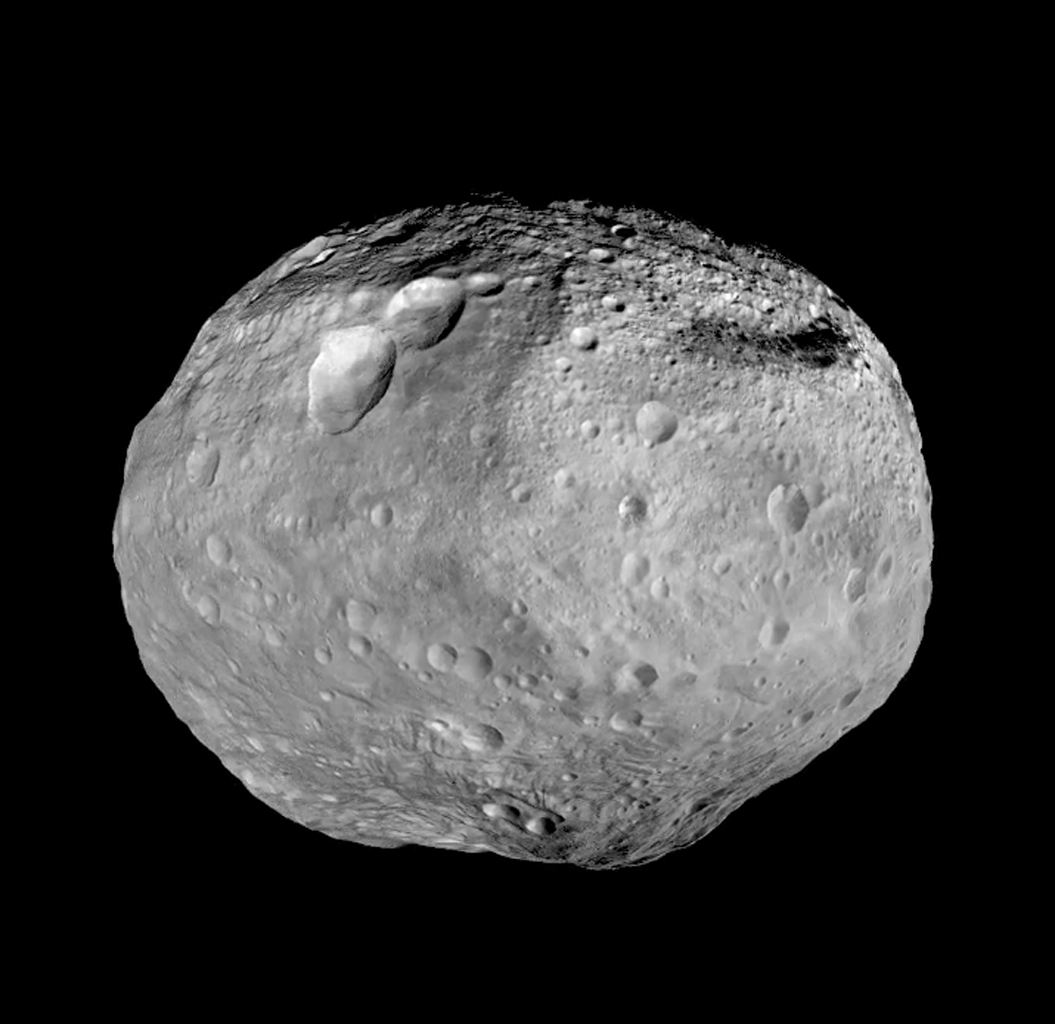
\includegraphics[width=0.95\textwidth]{../obr/vesta.jpg}
			\caption{Planetka \textit{(4) Vesta} --- druhé největší a~nejhmotnější těleso hlavního pásu planetek.} \label{fig:vesta}
			\end{subfigure}
			\begin{subfigure}[t]{0.55\textwidth}
			\centering
			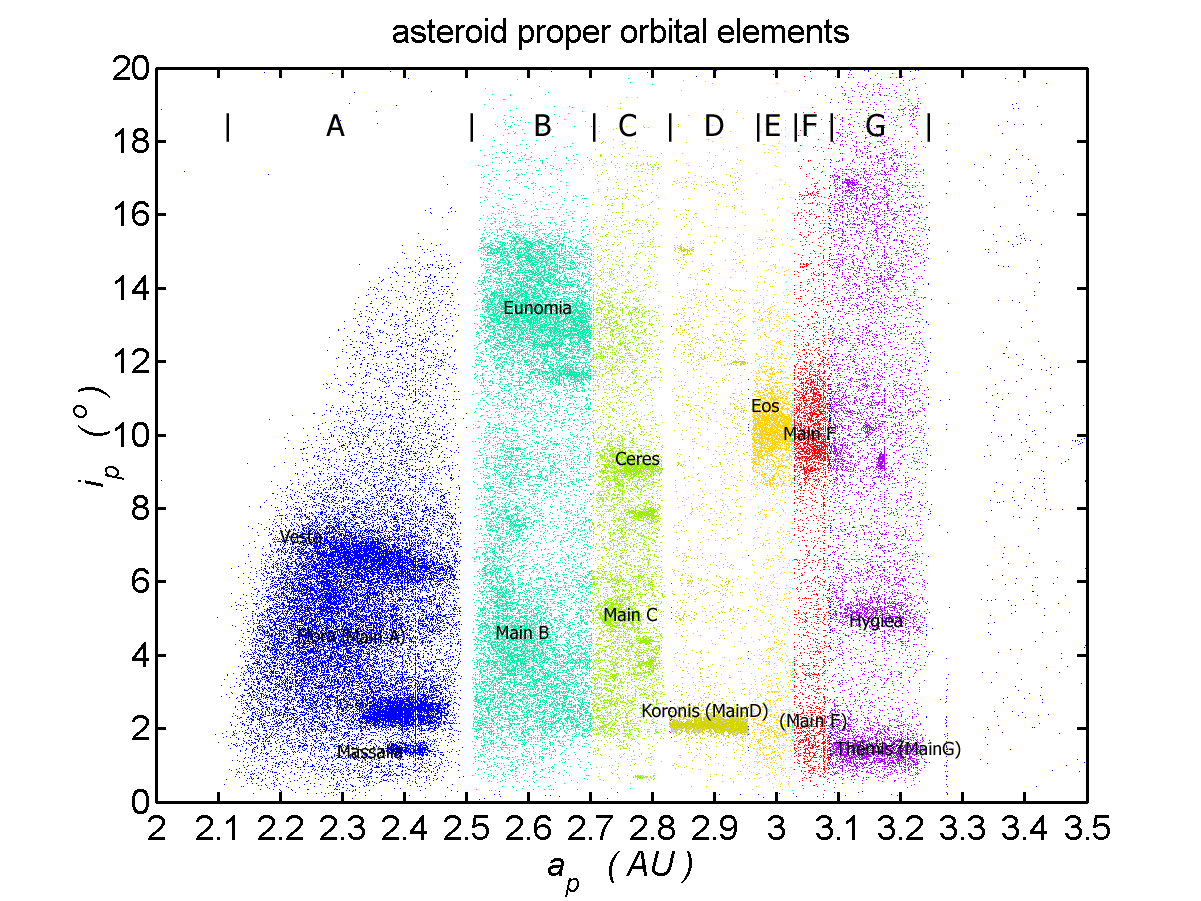
\includegraphics[width=1.0\textwidth]{../obr/mainbelt.png}
			\caption{Hlavní pás planetek v prostoru \textbf{vlastních elementů dráhy} --- vlastní hlavní poloosy $a_{\rm p}$ vlastní sklon $\sin I_{\rm p}$.} \label{fig:belt}
			\end{subfigure}
		\end{figure}
	\end{tcolorbox}

\vspace{\sep}

	\begin{tcolorbox}[title=Metody\phantom{Úy},height=0.665\vyskaA]

		Základním problémem nebeské mechaniky je \textbf{problém $N$ těles} --- vypočítat polohu těles, která na sebe vzájemně gravitačně působí v souladu s \textbf{Newtonovým gravitačním zákonem}.

		{\footnotesize
		\begin{align*} 
			\vec{F}_i = m_i\vec{a}_i &= -\sum_{\substack{j=1 \\ j\neq i}}^N G\frac{m_im_j}{\abs{\vec{r}_i-\vec{r}_j}^3}(\vec{r_i}-\vec{r_j})\,, \qquad{\rm pro}\ i\in\{1,\,2,\,\dots,\,N\} \\
			\vec{a}_i &= -\sum_{\substack{j=1 \\ j\neq i}}^N \frac{Gm_j}{\abs{\vec{r}_i-\vec{r}_j}^3}(\vec{r_i}-\vec{r_j})\,, \qquad{\rm pro}\ i\in\{1,\,2,\,\dots,\,N\} 
		\end{align*}}

K simulaci orbitálního vývoje využíváme \textbf{\it numerického integrátoru SWIFT}, který počítá s \textbf{Jarkovského jevem}, \textbf{YORP efektem}, \textbf{náhodnými srážkami} i \textbf{chaotickou difuzí}. Zde můžete vidět ilustraci jednodušší integrační metody --- \textbf{Eulerovy metody} --- která je ale pricipielně té naší podobná. 
		\begin{figure}[!htb]
			\centering 
			\begin{subfigure}[b]{0.45\textwidth}
			\centering 
			\asyinclude[width=1.0\textwidth]{../asy/f_euler.asy}
			\end{subfigure}
			\begin{subfigure}[b]{0.45\textwidth}
			\centering 
			\asyinclude[width=1.0\textwidth]{../asy/b_euler.asy}
			\end{subfigure}
			% \caption{Ilustrace dopředné Eulerovy integrační metody pro dvě tělesa. Jsou ukázány první tři iterace. Šedá křivka znázorňuje analytické řešení problému dvou těles.} \label{fig:euler}
		\end{figure}
		\vspace{-36pt}
		Podle pohybu planetky vzhledem ke Slunci můžeme určovat \textbf{elementy dráhy}. Ty se v průběhu času mění působením \textbf{perturbací} (např. gravitační působení ostatních planet), můžeme je tedy přes dlouhé úseky \uv{průměrovat} na \textbf{střední} a na \textbf{vlastní elementy dráhy}, přičemž druhé z nich jsou nepodléhají žádným periodickým silám.

		\begin{figure}
			\centering
			\begin{subfigure}[b]{0.49\textwidth}
			\centering
			\includegraphics[width=1.0\textwidth]{../obr/atOF}
			\end{subfigure}
			\begin{subfigure}[b]{0.49\textwidth}
			\centering
			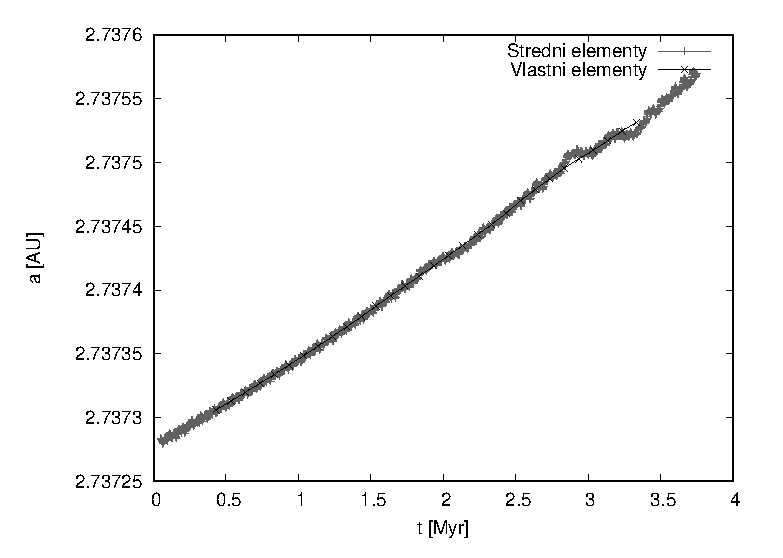
\includegraphics[width=1.0\textwidth]{../obr/atFP}
			\end{subfigure}
			\caption{\ Porovnání \textbf{oskulační} (aktuální) a \textbf{střední} hlavní poloosy (vlevo) a \textbf{střední} a~\textbf{vlastní} hlavní poloosy(vpravo) pro simulaci jedné planetky po dobu $3,76$ miliónů let.}
		\end{figure}
		\vspace{-48pt}
		\begin{tabularx}{\textwidth}{p{12cm}X}

		\

		K určení členů rodiny používáme \textbf{hierarchickou shlukovací metodu} (HCM) --- v prostoru $(a_{\rm p},\,e_{\rm p},\sin I_{\rm p})$ si zvolíme hraniční vzájemnou \uv{vzdálenost} těles $v_{\rm cutoff}$ (s jednotkami rychlosti), podle které pak určíme členy.

		{\footnotesize \begin{align*}
			v=na_{\rm p}\sqrt{C_a\left(\frac{\Delta a_{\rm p}}{a_{\rm p}}\right)^2+C_e(\Delta e_{\rm p})^2+C_i(\Delta \sin i_{\rm p})^2}
		\end{align*}}
		&
		\begin{figure}
			\centering
			\includegraphics[width=0.4\textwidth]{../obr/Nv}
			\caption{Závislost počtu členů rodiny \textit{Eunomia} na zvolené hraniční rychlosti $v_{\rm cutoff}$ při použití metody HCM. Počet členů prudce vzroste při přechodu z~$43$ na $44\,{\rm m/s}$, což je způsobené velkou vzdáleností prvního nejbližšího tělesa od mateřského \textit{(15) Eunomia}. Dále vzroste prudce při přechodu z~$46$ na $47\,{\rm m/s}$, což je způsobené splynutím s~rodinou Adeona.}
		\end{figure}
		\end{tabularx}

	\end{tcolorbox}

\vspace{\sep}

\end{column}

\begin{column}{2\sep}
\end{column}

\begin{column}{\main}
\begin{tcolorbox}[title=Výsledky\phantom{Úy},height=\vyskaB]

	\vspace{-1cm}
	\begin{textblock*}{35cm}(51.5cm,25.5cm) % {block width} (coords) 
		K určení rodiny \textit{Eunomia} jsme použili metodu HCM s hodnotou $v_{\rm cutoff}=44\,{\rm m/s}$. Dále jsme odstranili \textbf{přimísená tělesa} pomocí závislosti unášení ve \textbf{vlastní hlavní poloose} $\Delta a_{\rm p}$ na \textbf{absolutní hvězdné velikosti} $H$ a pomocí dvou spektroskopických metod --- závislosti \textbf{albed} $p_{\rm V}$ a $p_{\rm IR}$ a závislosti \textbf{barevných indexů} $a^*$ a $i-z$. Před odstraněním činil počet planetek 6503, po použití všech metod~6184.
	\end{textblock*}
	\begin{figure}[!htb]
		\begin{subfigure}[b]{0.3\textwidth}
			\centering
			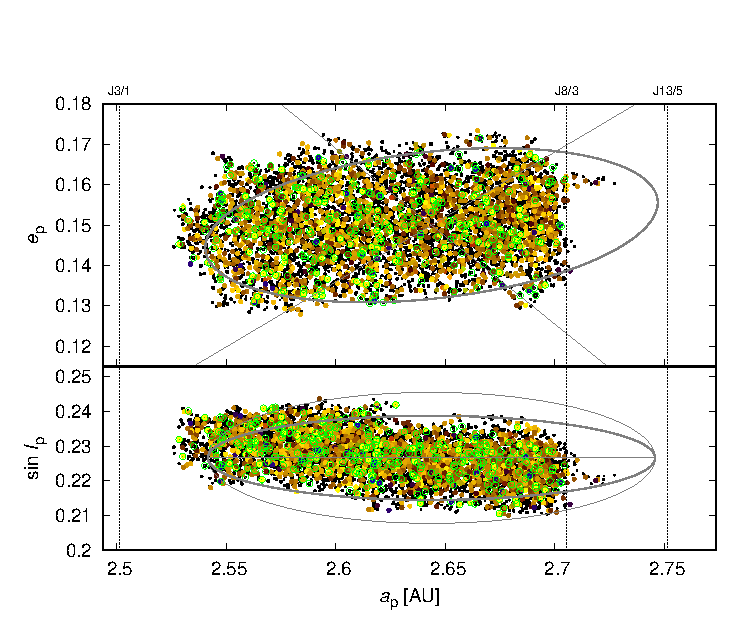
\includegraphics[width=1.0\textwidth]{../obr/ae_ai_wise}
			\caption{Pozorovaná rodina \textit{Eunomia} určená HCM s hodnotou $v_{\rm cutoff} = 44\,{\rm m/s}$ v~rovině \textbf{vlastní hlavní poloosy} $a_{\rm p}$ a~\textbf{vlastní excentricity} $e_{\rm p}$ (nahoře) a~v~rovině \textbf{vlastní hlavní poloosy} $a_{\rm p}$ a~\textbf{vlastního sklonu} $\sin I_{\rm p}$ (dole). Barevná škála odpovídá \textbf{albedu} $p_{\rm V}$ a~$p_{\rm IR}$ z~katalogu WISE \cite{nugent15}. Nápisy J3/1, J8/3 a~J13/5 označují polohu \textbf{rezonancí středního pohybu} s~\textit{Jupiterem}. Šedé elipsy a~úsečky (degenerované elipsy) naznačují předpokládaný tvar rodiny, při rozpadu v bodě oběžné dráhy s hodnotami \textbf{pravé anomálie} $f=0^\circ,\,90^\circ,\,180^\circ$ (nahoře) a~jejího součtu s \textbf{argumentem pericentra} $\omega+f=0^\circ,\, 50^\circ,\, 90^\circ$ (dole), kde elipsou zvolenou pro další výpočety je elipsa pro hodnoty $f=90^\circ$ a~$\omega+f=50^\circ$.}
			\label{fig:ae_ai_wise}
		\end{subfigure}
		\begin{subfigure}[b]{0.26\textwidth}
			\centering
			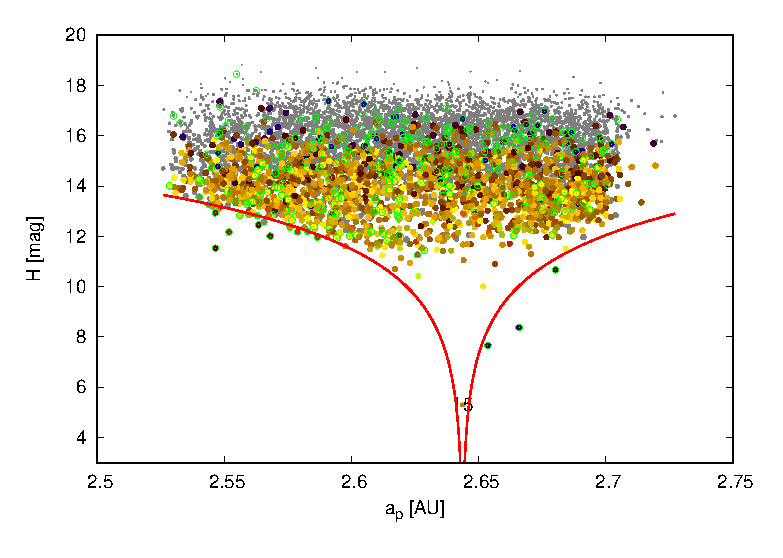
\includegraphics[width=1.0\textwidth]{../obr/aH_wise}
			\caption{Pozorovaná rodiny \textit{Eunomia} v~rovině \textbf{vlastní hlavní poloosy} $a_{\rm p}$ a~\textbf{absolutní hvězdné velikosti} $H$. Lze pozorovat typický tvar \uv{V}, který je způsobem počátečním \textbf{rychlostním polem} a~\textbf{Jarkovského jevem}, jenž je ještě zesílen vlivem \textbf{YORPu}, což způsobuje zvýšenou koncentraci malých planetek při okrajích rodiny.}
		\end{subfigure}
		\begin{subfigure}[b]{0.2\textwidth}
			\centering
			\includegraphics[width=1.0\textwidth]{../obr/pV_pIR-crop}
			\caption{\textbf{Albeda} $p_{\rm V}$ (ve viditelném spektru) a~$p_{\rm IR}$ (v~infračerveném) z~katalogu WISE. Barvy neodpovídají reálnému zbarvení. Pro vyřazení \textbf{přimísených těles} touto metodou byly zvoleny hraniční hodnoty $0,05 \leq p_{\rm V} \leq 0,4$.}
		\end{subfigure}
		\begin{subfigure}[b]{0.2\textwidth}
			\centering
			\includegraphics[width=1.0\textwidth]{../obr/astar_iz-crop}
			\caption{\textbf{Barevné indexy} $a^*$ a~$i-z$ z~katalogu Sloan \cite{ivezic01}. Barvy neodpovídají reálnému zbarvení. Pro vyřazení \textbf{přimísených těles} byly zvoleny hraniční hodnoty $0\leq a^* \leq 0,3$ a~$-0,3\leq i-z \leq 0,3$.
% \\
% \
}
		\end{subfigure}
	\end{figure}

	\begin{tabularx}{\textwidth}{p{0.6\textwidth}X}

\

Při vytváření \textbf{syntetické} populace planetek jsme částicím přiřadili \textbf{průměry}, \textbf{albeda} a \textbf{orientace rotačních os} (vliv na \textbf{Jarkovského jev}) podle pozorované rodiny nebo náhodně. U průměrů jsme zohlednili \textbf{rozdělení velikostí} a při zpracovávání simulace jsme rozdělení korigovali tak, aby odpovídalo pozorovanému.

Dále jsme částicím přiřadili \textbf{úvodní rychlosti} jako při \textbf{izotropním rozpadu} v bodě oběžné dráhy s hodnotami $f=90^\circ$ a $\omega+f=50^\circ$.

Po dobu \textbf{jedné miliardy let} jsem simulovali populaci 6210 částic s tím, že přibližně v půlce došlo ke ztrátě dat. Simulace byla spuštěna na \textit{výpočetním clusteru Astronomického ústavu Univerzity Karlovy} a celkově se spotřebovalo 23040 \textbf{CPU hodin}. Protože jsme z~ladících důvodů nechali ukládat nejen \textbf{vlastní}, ale i~\textbf{střední} elementy, je celkový objem \textbf{binárních dat} roven $164\,{\rm GB}$.

	&

	\begin{figure}
		\centering
		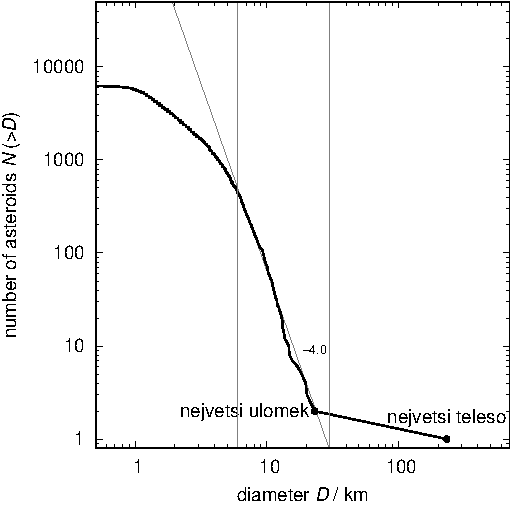
\includegraphics[width=0.17\textwidth]{../obr/size_distribution-crop}
		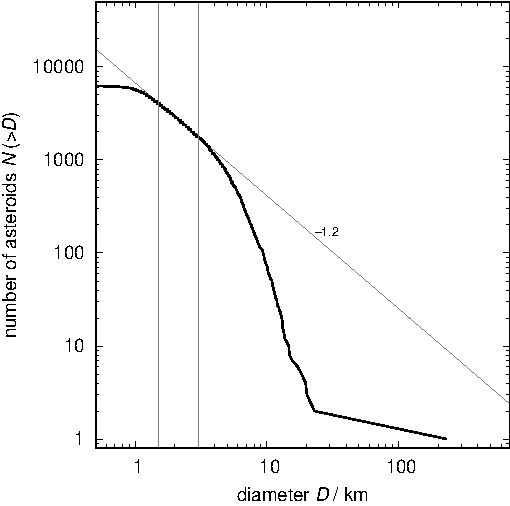
\includegraphics[width=0.17\textwidth]{../obr/size_distribution_SMALLD-crop}
	\caption{\textbf{Histogram} četnosti velikostí planetek rodiny \textit{Eunomia}, kde veličina $N({>}D)$ označuje počet planetek s~\textbf{průměrem} větším než $D$. Jedná se o~\textbf{logaritmický graf} $(\log D,\,\log N({>}D))$, na kterém lze vztah mezi danými veličinami aproximovat přímkou, což znamená, že vztah mezi veličinami $D$ a~$N({>}D)$ je \textbf{mocninný}. Vodorovná část zcela vlevo je způsobena observační nedostatečností. Změna sklonu přímky prvního intervalu $D$ (vlevo, $q=-4$) na druhý interval $D$ (vpravo, $q=-1,2$) je důsledkem jednak prvotního rozpadu a~jednak druhotného vývoje --- tělesa se nadále srážejí, vytvářejí menší tělesa, která snáze opouštějí rodinu.}
		\label{fig:sfd}
	\end{figure}
	\end{tabularx}

	\vspace{-1.5cm}
	\begin{figure}[t]
		\centering
		\begin{subfigure}[t]{0.33\textwidth}
			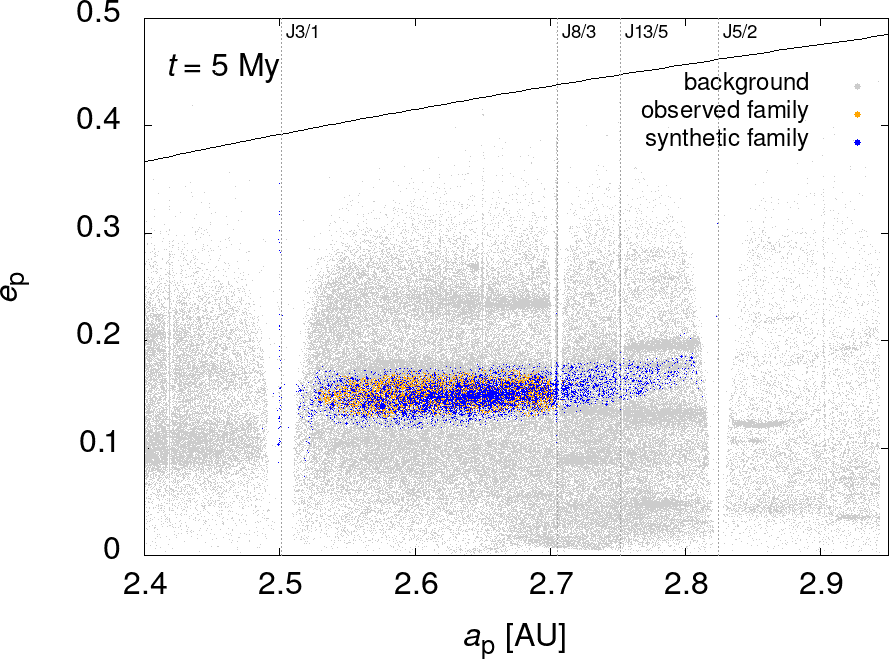
\includegraphics[width=0.49\textwidth]{../obr/ae_5t_trans.png}
			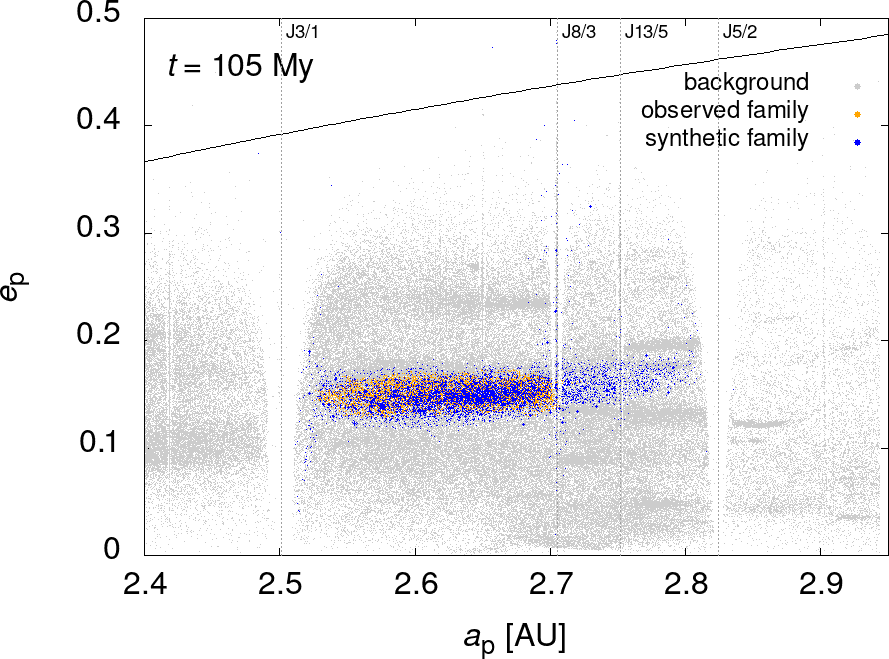
\includegraphics[width=0.49\textwidth]{../obr/ae_105t_trans.png}\\
			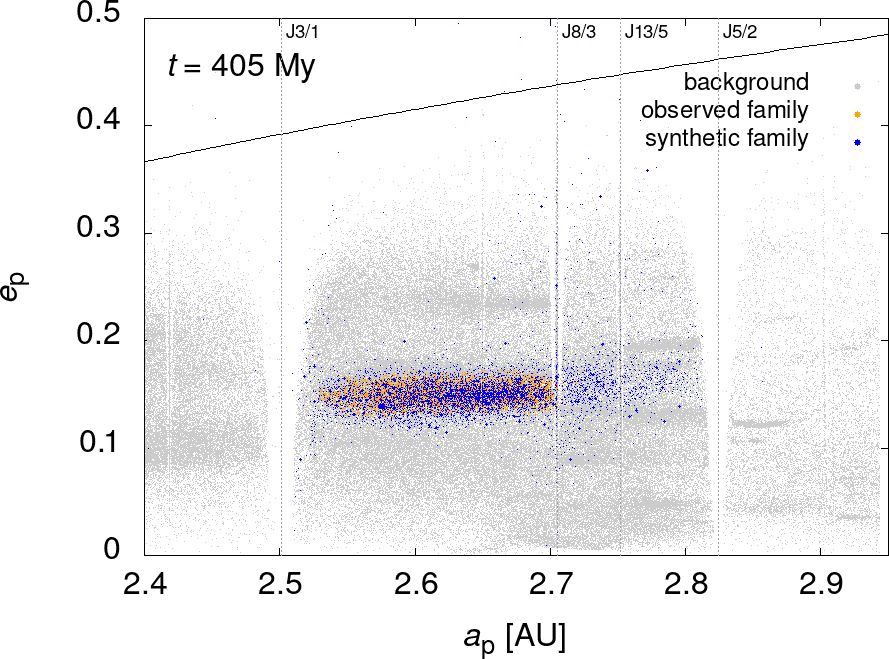
\includegraphics[width=0.49\textwidth]{../obr/ae_405t_trans.png}
			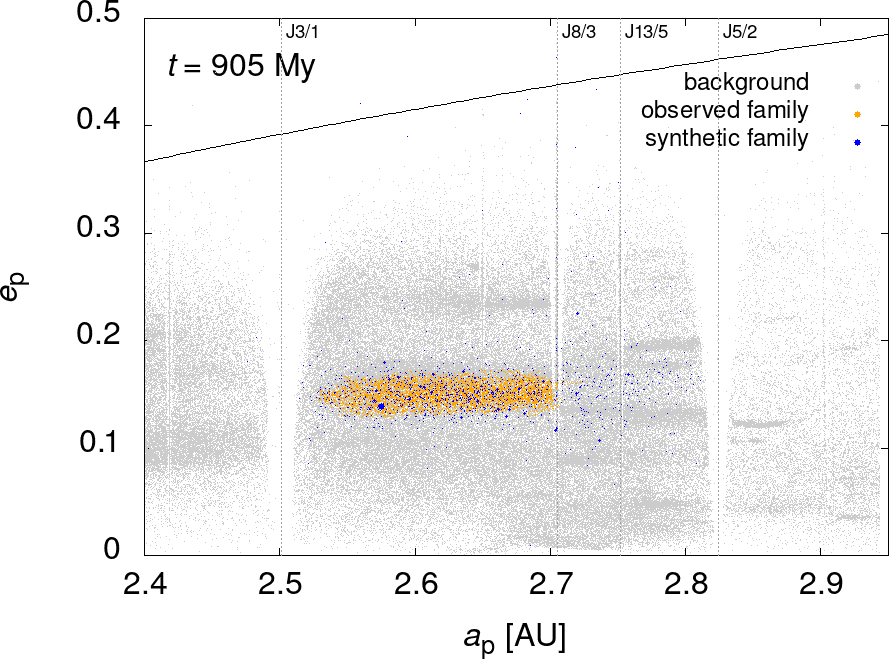
\includegraphics[width=0.49\textwidth]{../obr/ae_905t_trans.png}
		\end{subfigure}
		\begin{subfigure}[t]{0.33\textwidth}
			\centering
			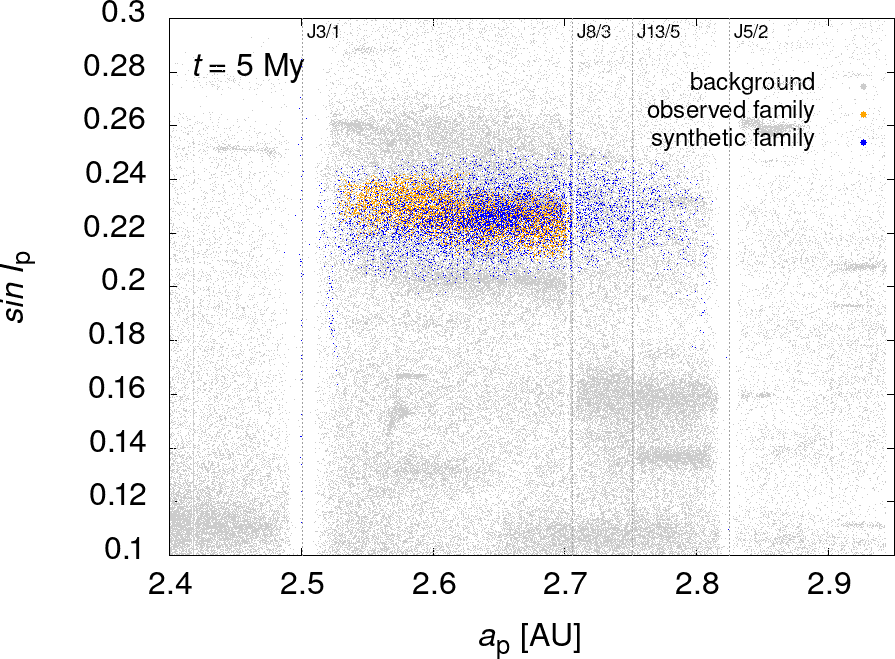
\includegraphics[width=0.49\textwidth]{../obr/ai_5t_trans.png}
			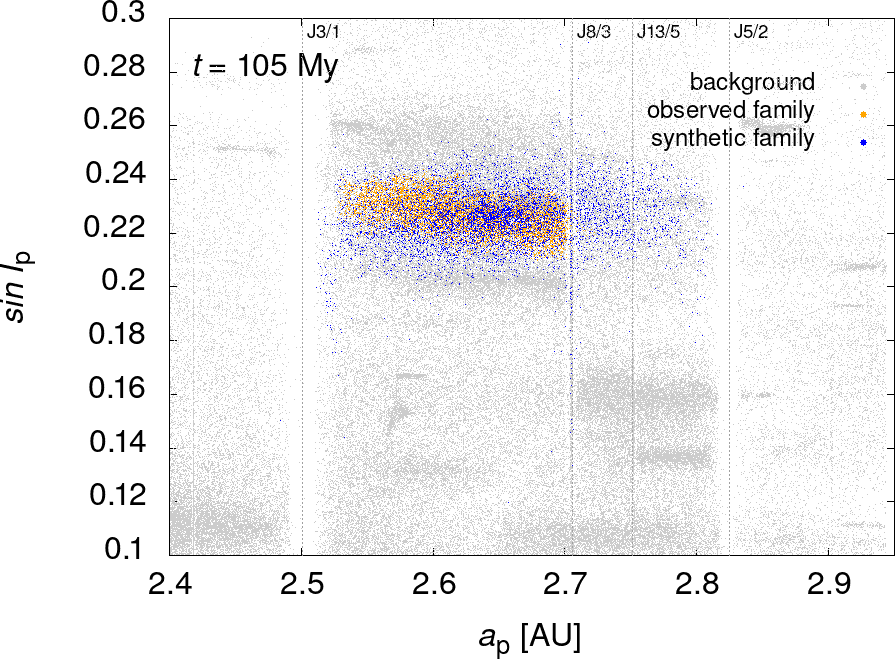
\includegraphics[width=0.49\textwidth]{../obr/ai_105t_trans.png}\\
			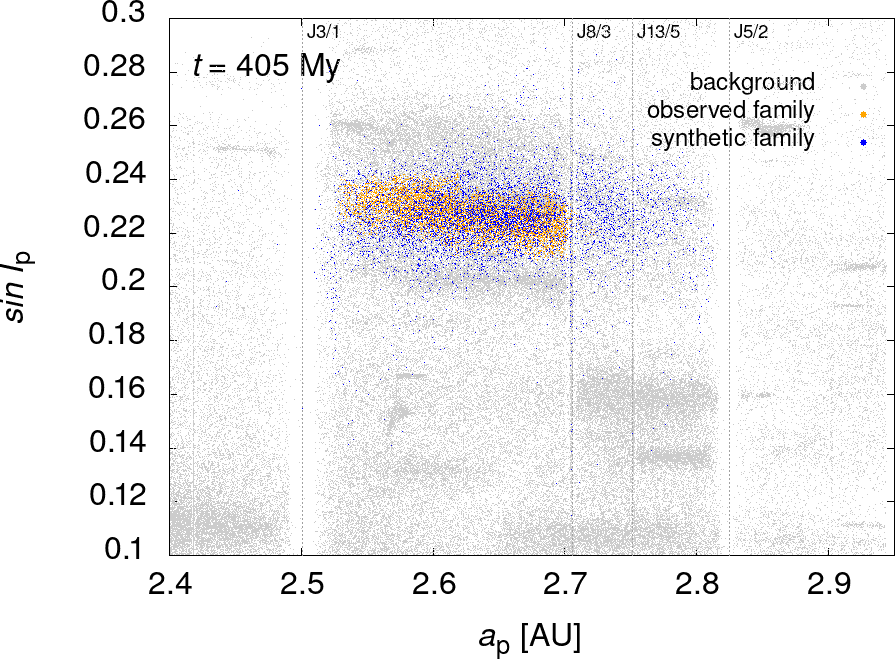
\includegraphics[width=0.49\textwidth]{../obr/ai_405t_trans.png}
			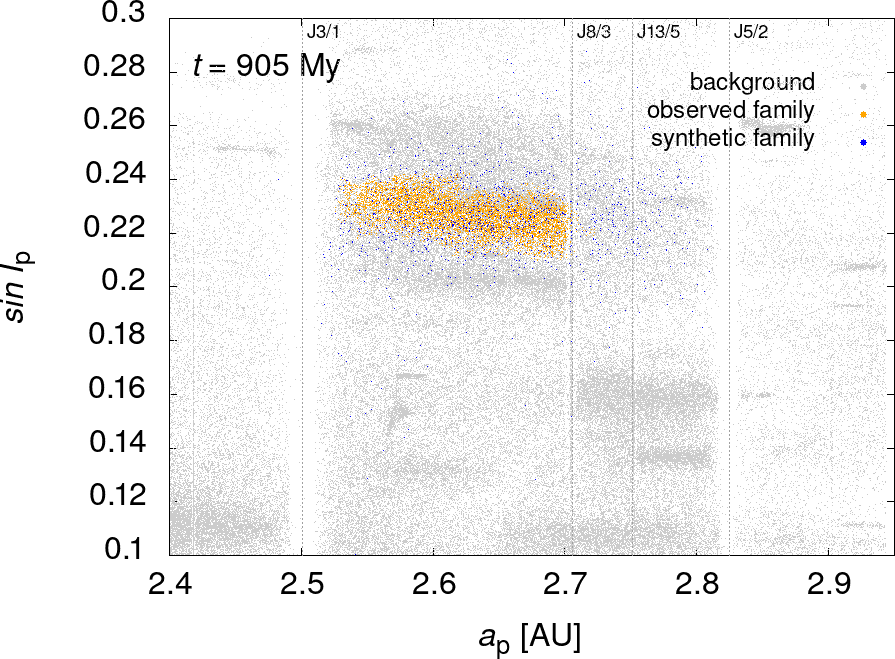
\includegraphics[width=0.49\textwidth]{../obr/ai_905t_trans.png}
		\end{subfigure}
		\begin{subfigure}[t]{0.33\textwidth}
			\centering
			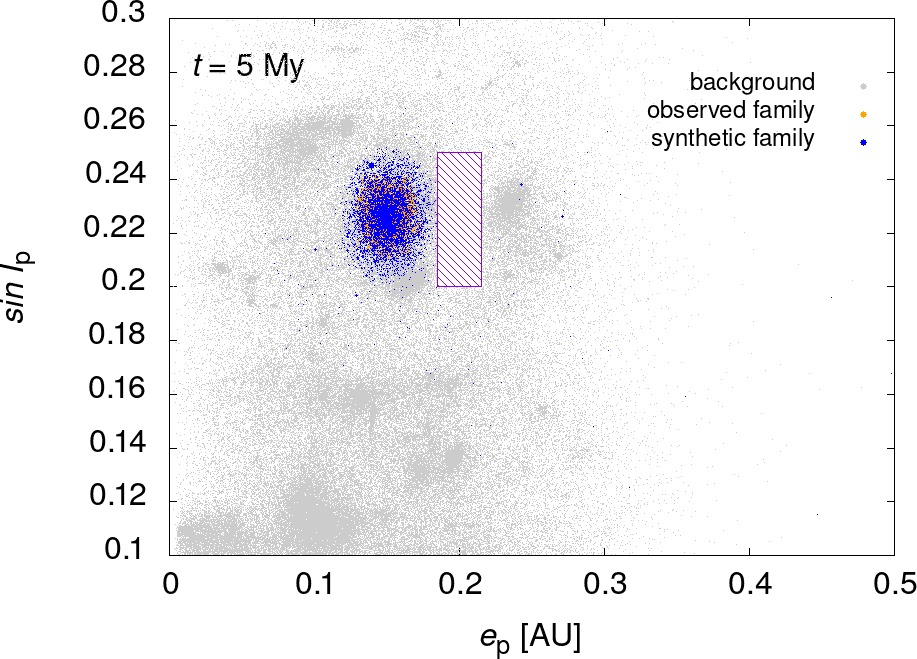
\includegraphics[width=0.49\textwidth]{../obr/ei_5t_trans.png}
			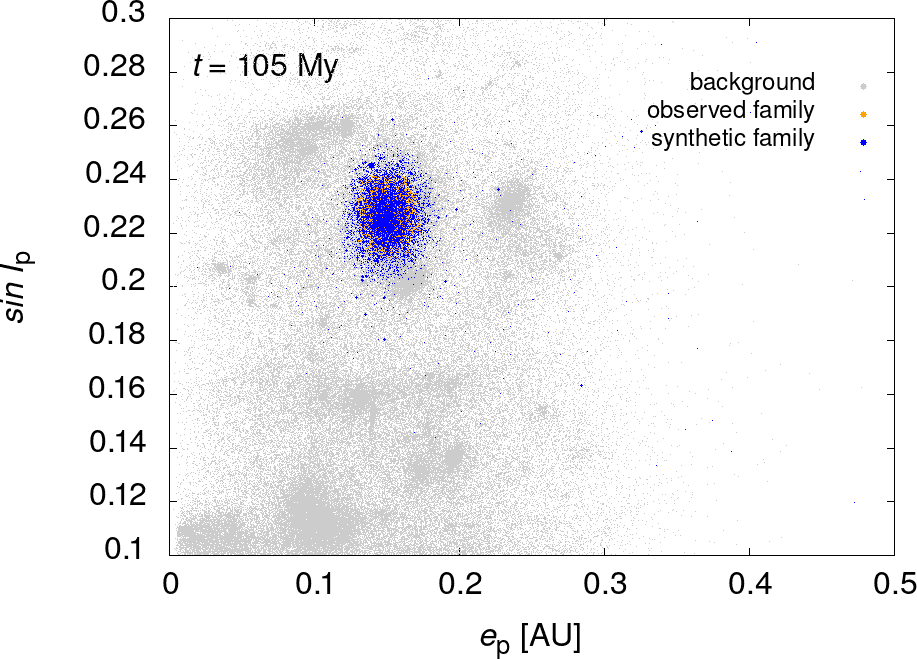
\includegraphics[width=0.49\textwidth]{../obr/ei_105t_trans.png}\\
			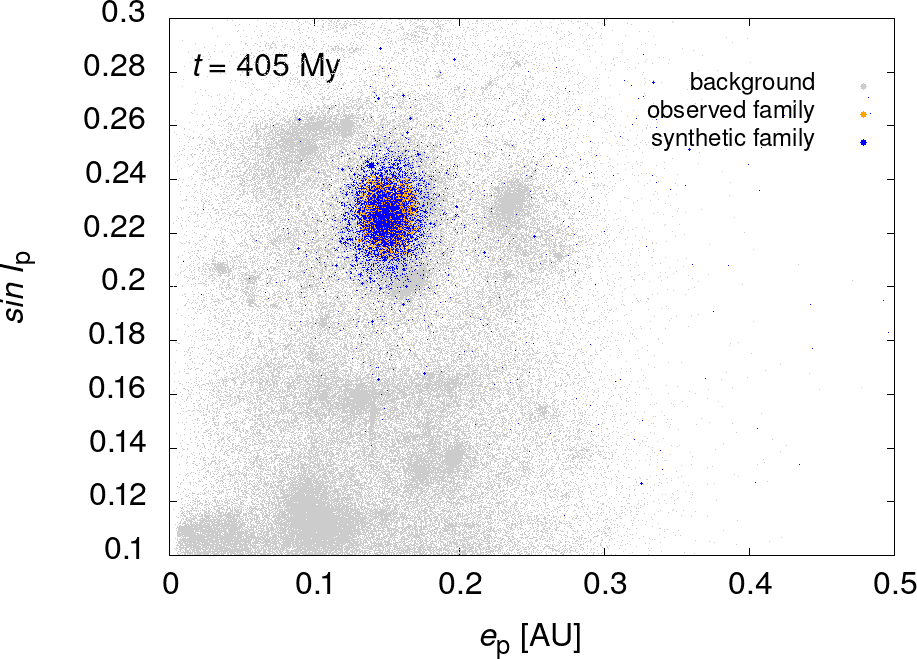
\includegraphics[width=0.49\textwidth]{../obr/ei_405t_trans.png}
			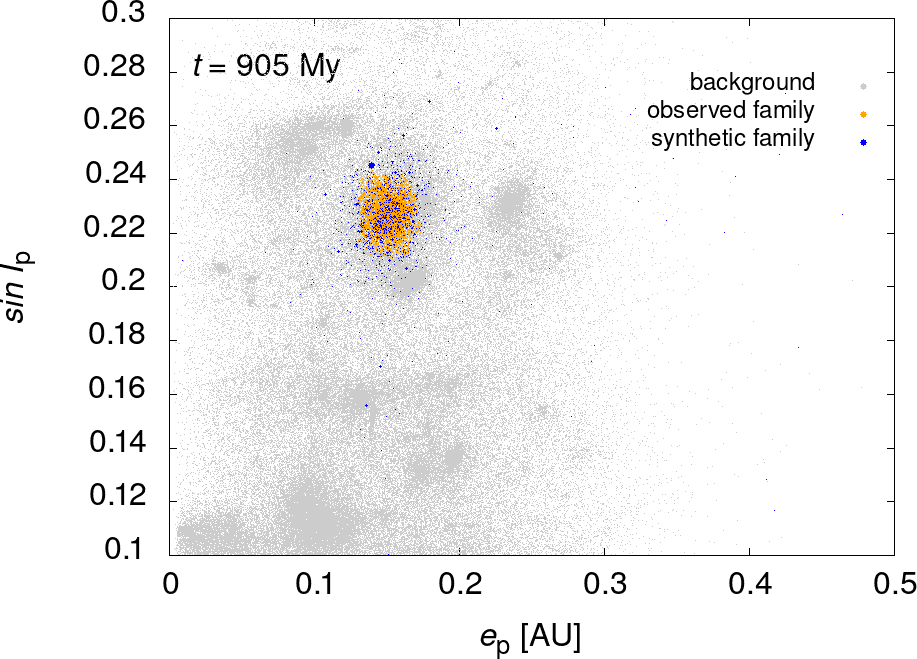
\includegraphics[width=0.49\textwidth]{../obr/ei_905t_trans.png}
		\end{subfigure}
			\caption{Výsledky simulace v~prostorech $(a_{\rm p},\,e_{\rm p})$, $(a_{\rm p},\,\sin I_{\rm p})$ a  $(e_{\rm p},\,\sin I_{\rm p})$ v~časech postupně $t=5,\,105,\,405,\,905$ miliónů let. Modré body označují \textbf{simulovanou} rodinu, žluté body \textbf{pozorovanou} rodinu identifikovanou HCM a~šedé body \textbf{pozadí} a~jiné okolní rodiny. Jsou také značeny nejvýznamnější \textbf{rezonance} s~\textit{Jupiterem} J3/1, J8/3, J13/5 a~J5/2. Černá křivka nahoře označuje hranici oblasti, kde je hlavní poloosa a~excentricita tělesa taková, že dráha kříží dráhu \textit{Marsu}. Podobná hranice existuje i~pro \textbf{Jupiter}, ale ta se nachází mimo tyto grafy (přibližně kolem $e=0,65$). Fialový obdélník označuje oblast vybranou pro vzorek populace \textbf{pozadí}.} \label{fig:ae_sim}
	\end{figure}

Kvůli specifickému výpočtu \textbf{vlastních elementů dráhy} z~počátečních rychlostí můžeme v~čase 5 miliónů let pozorovat mírně nesymetrický tvar simulované~rodiny. 

Lze vidět vliv \textbf{rezonancí středního pohybu} J3/1, J5/2, J8/3 a J13/5 --- v jejich blízkosti se \textbf{excentricity} planetek začnou zvyšovat, až se dostanou do oblasti, kde kříží dráhy \textit{Marsu} nebo \textit{Jupitera}, což znamená, že se planetka dříve nebo později některé z~těchto planet přiblíží a~její \textbf{hlavní poloosa} se náhle změní. \textbf{Rezonance} J8/3 a~J13/5 jasně rozdělují planetky do oblastí, ze kterých planetky zřídkakdy vystupují. Na prvním obrázku jsou data již zprůměrována z~prvních $10$ miliónů let, takže můžeme vidět, že se planetky, které se zřejmě na počátku nacházely v~blízkosti \textbf{rezonancí} J3/1, J8/3 a~J13/5, stihly rozptýlit a~narušily tak jinak zatím pravidelný tvar rodiny. Potvrzuje se, že \textbf{rezonance} J8/3 je silnější než \textbf{rezonance} J13/5 (planetky v~její blízkosti se v~čase 105 miliónů let rozšířily do pásu o~velikosti $0,05<e_{\rm p}<0,5$, zatímco v~blízkosti \textbf{rezonance} J13/5 pouze do pásu o~velikosti $0,1<e_{\rm p}<0,23$)

Na grafu $(a_{\rm p},\,\sin I_{\rm p})$ můžeme pozorovat mírné \uv{naklonění} pozorované rodiny (část pod $a\approx2,62\,{\rm AU}$ má vyšší sklon $I_{\rm p}$), čehož si na rodině simulované bohužel zatím všimnout nemůžeme.

\newlength{\chiwidth}
\setlength{\chiwidth}{0.2\textwidth}
\begin{tabularx}{\textwidth}{Xp{30cm}}
	\begin{figure}
		\centering
		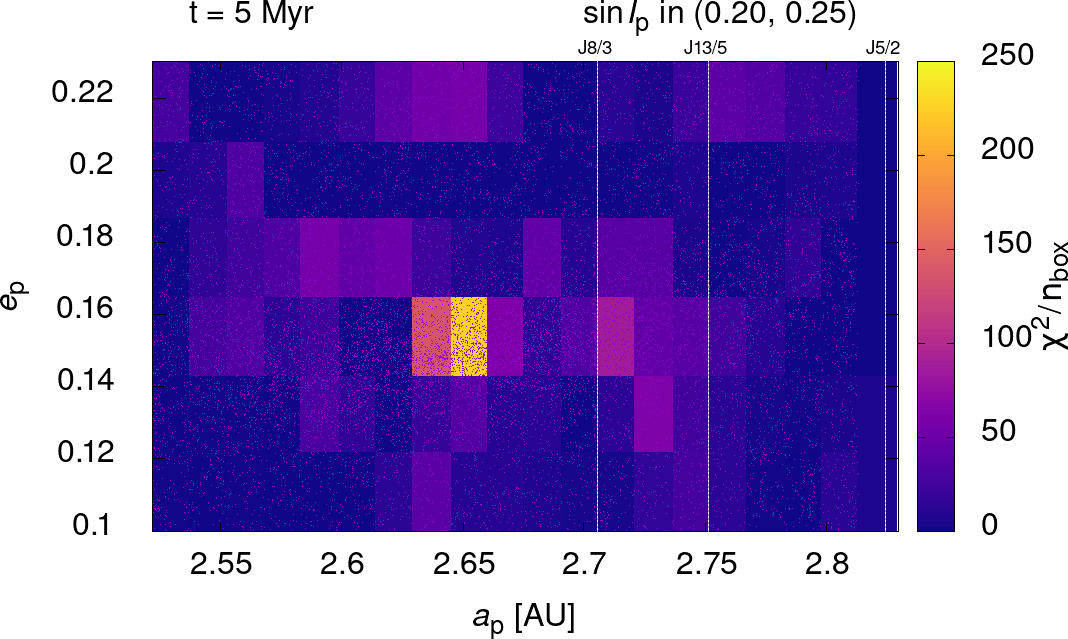
\includegraphics[width=\chiwidth]{../obr/ae_chi_0006t_trans.png}
		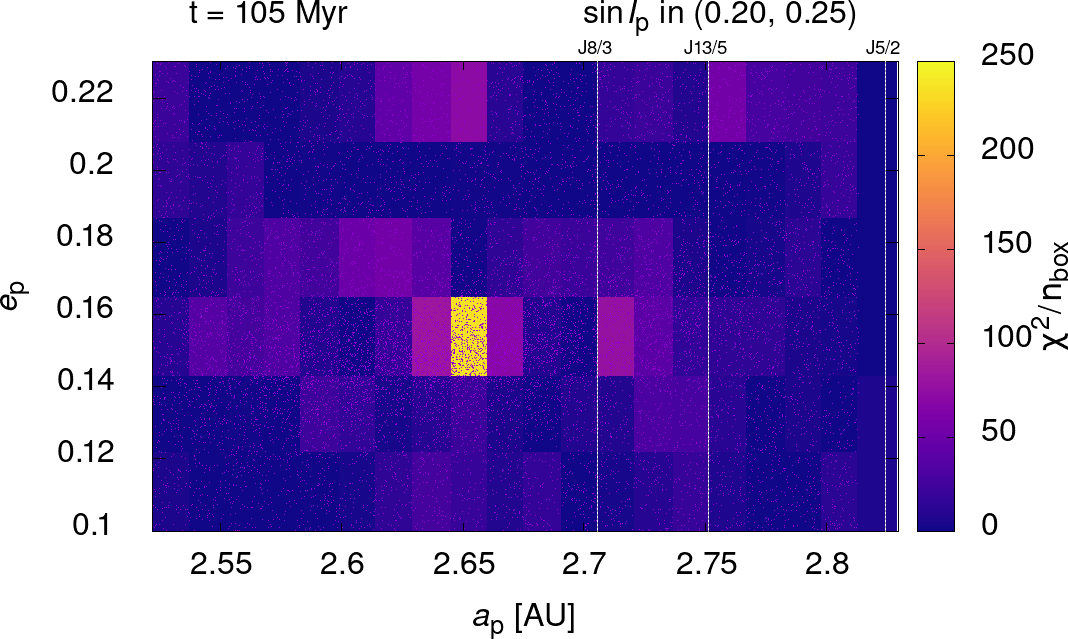
\includegraphics[width=\chiwidth]{../obr/ae_chi_0106t_trans.png}\\
		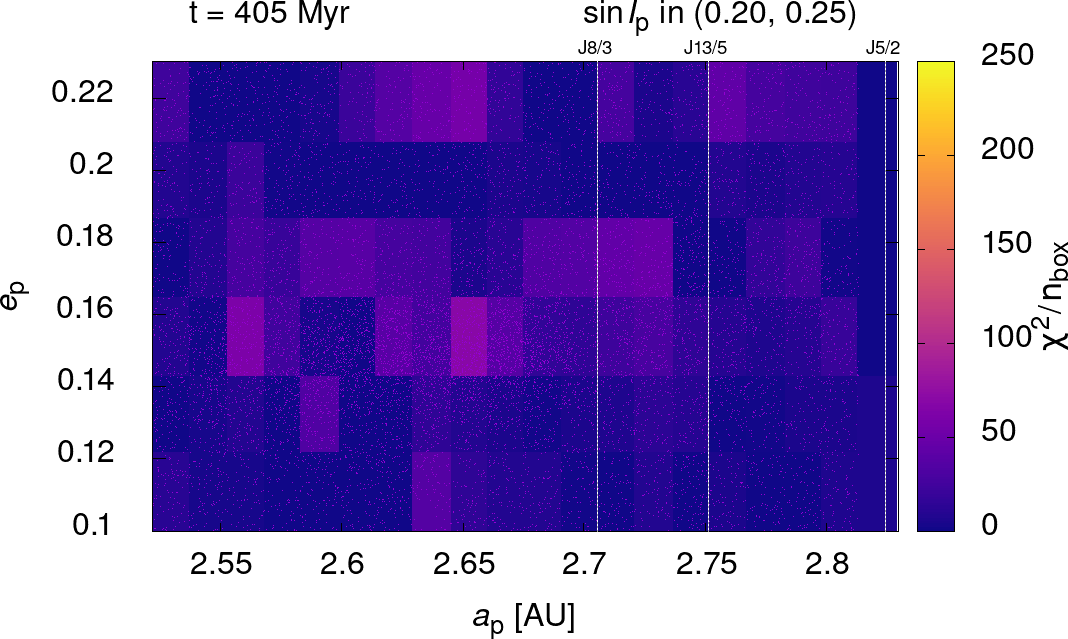
\includegraphics[width=\chiwidth]{../obr/ae_chi_0406t_trans.png}
		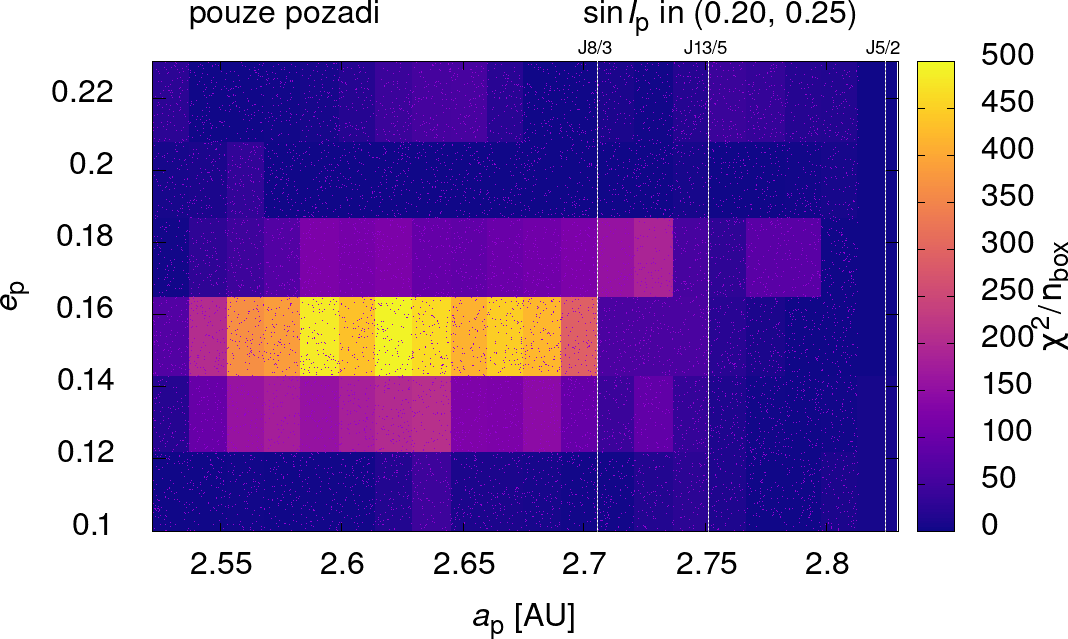
\includegraphics[width=\chiwidth]{../obr/ae_chi_emptyt_trans.png}
		\caption{Hodnota \textbf{chi kvadrátu} $\chi^2$ pro každý \textbf{box} v~prostoru $(a_{\rm p},\,e_{\rm p})$. Na prvních třech obrázcích lze vidět rozdělení \textbf{chi kvadrátu} pro $t=5,\,105,\,405$ miliónů let, na posledním obrázku lze vidět rozdělení \textbf{chi kvadrátu} při vygenerování pouze \textbf{pozadí} bez použití částic simulované rodiny. Tečky označují \textbf{syntetickou} populaci i~s~přidaným \textbf{pozadím}.} \label{fig:ae_chi2}
	\end{figure}
&

\ 

K~odhadu \textbf{stáří rodiny} jsme použili metodu nazvanou příznačně \uv{\textit{blackbox}} popsanou v~\cite{broz19}, která funguje na principu rozdělení planetek jak pozorované, tak simulované rodiny do \uv{boxů} v~prostoru $(a_{\rm p},\,e_{\rm p},\,\sin I_{\rm p})$ a~následném porovnání počtů pozorovaných a~simulovaných planetek v~jednotlivých \textbf{boxech}. Simulovanonou populaci ještě \uv{smícháváme} se vzorkem \textbf{pozadí}, přičemž dodržuje \textbf{rozdělení velikostí}. 

Na tento jednoduchý princip je pak použita standardní statistická metoda rozdělení \textbf{chí kvadrátu} $\chi^2$ --- pro každý \textbf{box} vypočteme jeho příspěvek k~$\chi^2$ jako
\begin{align*}
	\frac{(N_{\rm sim}-N_{\rm obs})^2}{N_{\rm sim}+N_{\rm obs}}\,,
\end{align*}
kde $N_{\rm sim}$, resp.\ $N_{\rm obs}$ označuje počet simulovaných, resp. pozorovaných těles v~daném \textbf{boxu}. Výslednou hodnotu $\chi^2$ potom dostaneme prostým sečtením všech příspěvků.

Můžeme vidět, že nejvíce se odlišuje jádro rodiny kolem $2,65\,{\rm AU}$ (moc \textbf{syntetických} částic) a oblast nalevo od jádra v~oblasti $a_{\rm p}\in(2,55\,{\rm AU};\,2,5\,{\rm AU})$ a~$e_{\rm p}\in(0,14;\,0,16)$ (málo \textbf{syntetických} těles). Kvůli silné \textbf{kontaminaci} rodinou \textit{Adeona} v oblasti $0,16<e<0.18$ jsme byli nuceni pozorované členy této rodiny ručně odstranit\end{tabularx}
\end{tcolorbox}
\vspace{\sep}
\end{column}

\begin{column}{2\sep}
\end{column}

\begin{column}{\side}
\begin{tcolorbox}[title=Závěry\phantom{Úy},height=0.38\vyskaC]
	\begin{figure}
		\centering
		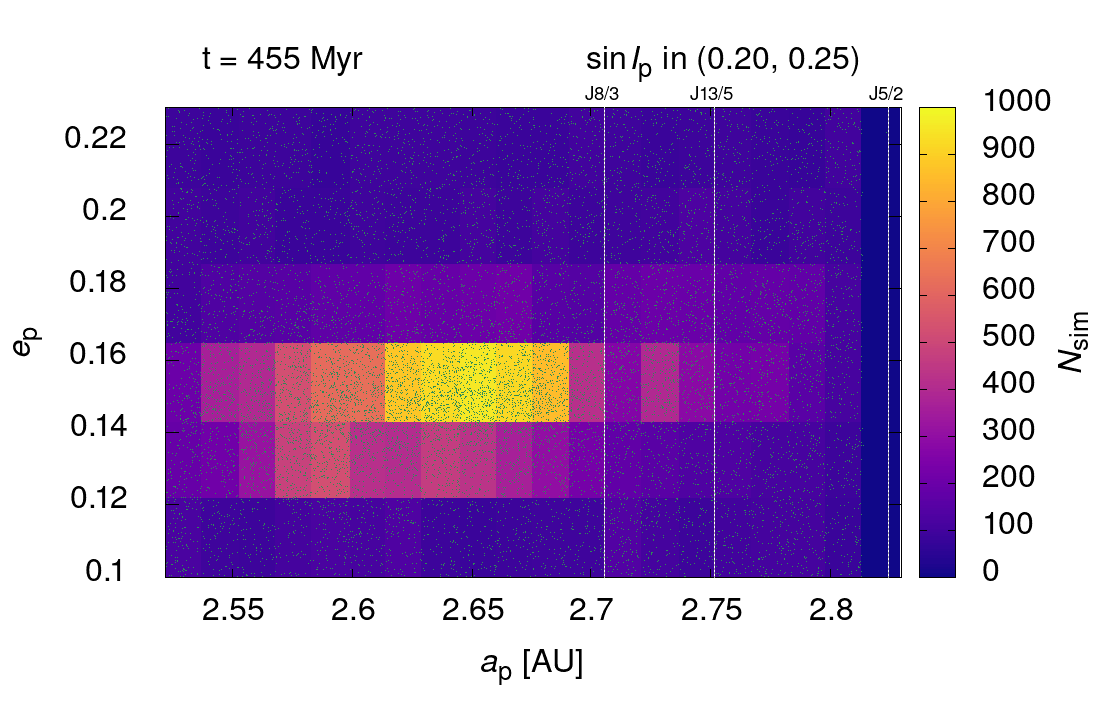
\includegraphics[width=0.49\textwidth]{../obr/ae_scl_trans.png}
		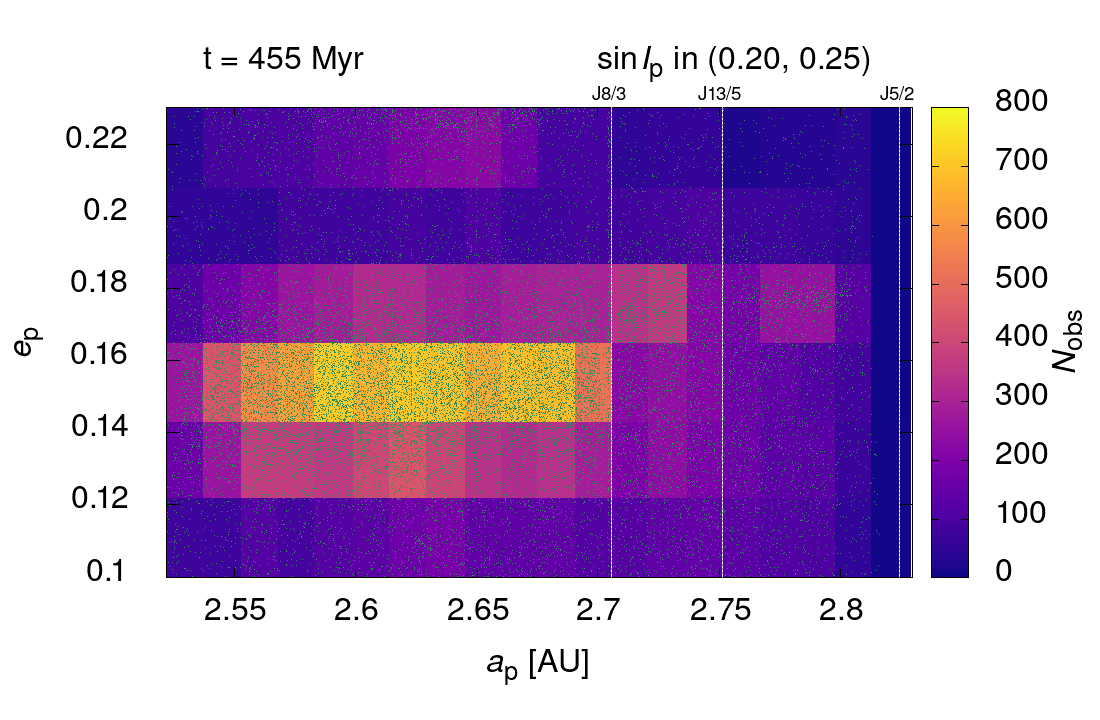
\includegraphics[width=0.49\textwidth]{../obr/ae_obs_trans.png}
		\caption{Graf $(a_{\rm p}, e_{\rm p})$ pro simulovanou (vlevo) a~pozorovanou (vpravo) rodinu \textit{Eunomia} v~čase $t=455$ miliónů let, kdy byla hodnota \textbf{chí kvadrátu} nejlepší. Tentokrát barevná škála označuje počet těles v~daném \textbf{boxu}.}
	\end{figure}

	Na obrázku můžeme vidět simulovanou a~pozorovanou rodinu \textit{Eunomia} v~okamžiku, kdy jsme dostali nejmenší hodnotu $\chi^2=11,9$, tedy naše data se nejvíce přibližovala realitě. Stále lze ale pozorovat nějaké nedostatky --- kromě již zmíněných můžeme poukázat na oblast $a_{\rm p}\in(2,7\,{\rm AU};\,2,75\,{\rm AU}),\ e_{\rm p}\in(0,16;\,0,18)$, kde se nachází velmi malá rodina příslušná planetce $(53546)\ 2000\,BY6$, se kterou jsme v~naší simulaci, stejně jako s~ostatními menšími rodinami, nepočítali.

	Podařilo se nám vysvětlit většinu \textbf{struktur}, které lze na našich grafech v prostorech $(a_{\rm p},\,e_{\rm p})$, $(a_{\rm p},\,\sin I_{\rm p})$ a  $(e_{\rm p},\,\sin I_{\rm p})$. Jediné, co zůstává nevysvětlené, je \textbf{kompaktnost jádra} simulované rodiny a~\textbf{absence částic} ve~oblasti \uv{nalevo} ($a_{\rm p}<2,57\,{\rm AU}$) od středu rodiny na grafu $(a_{\rm p},\,e_{\rm p})$. Tyto jevy bohužel musíme připsat \textbf{nedostatečně dlouhému časovému úseku}, po který jsme rodinu \textit{Eunomia} simulovali --- velice pravděpodobně tedy rodina \textit{Eunomia} \textbf{není mladší} než $500$ miliónů let.
\end{tcolorbox}
\vspace{\sep}
\begin{tcolorbox}[title=Budoucí práce\phantom{Úy},height=0.3\vyskaC]
	\begin{figure}
		\centering
		\includegraphics[width=0.5\textwidth]{../obr/chi2.eps}
	\end{figure}
	Lze pozorovat klesající trend \textbf{chí kvadrátu}, v~budoucnu tedy plánujeme simulovalat rodinu \textit{Eunomia} po \textbf{delší dobu} (4 miliardy let). Pravděpodobně dostaneme nějakou minimální hodnotu \textbf{chí kvadrátu}, čímž budeme schopni přesně určit \textbf{stáří} rodiny \textit{Eunomia}. Další možností výzkumu je analýza \textbf{okolních rodin}, zejména rodiny \textit{Adeona}. Přesné určení počtu jejích členů a~stáří by nám pomohlo v~analýze rodiny \textit{Eunomia}, mohli bychom např. v~momentu rozpadu rodiny \textit{Adeona} její částice do simulace přidat.

	Po \textbf{prodloužení dlouhodobé simulace} plánujeme \textbf{publikaci} výsledků v~odborném časopisu (\textit{Icarus}).

\end{tcolorbox}
\vspace{\sep}
\begin{tcolorbox}[title=Reference\phantom{Úy},height=0.32\vyskaC]
	\printbibliography

	\tcblower

	\newrefsection{}
	\setbeamertemplate{bibliography item}[book]
	\nocite{fmt}
	\nocite{murray00}
	\nocite{brozphd}
	\printbibliography
\end{tcolorbox}
\end{column}

\begin{column}{\sep}
\end{column}

\end{columns}
\end{frame}
\end{document}
